% !TEX program = lualatex
\documentclass{article}
\usepackage{fontspec}
\usepackage{luatexja-fontspec}
\usepackage{luatexja-ruby} % ルビを使用する場合に必要
\usepackage{graphicx}
\usepackage{listings}
\usepackage{amsmath}
\usepackage[top=25truemm,bottom=20truemm,left=20truemm,right=20truemm]{geometry}
%\usepackage{xcolor}

% フォントの設定
%\setmainfont{Noto Serif JP}    % 通常の明朝体
%\setsansfont{Noto Sans JP}     % 通常のゴシック体
%\setmonofont{Noto Sans Mono JP} % 等幅フォント
%\setmainjfont{Noto Serif JP}   % 日本語の明朝体
%\setsansjfont{Noto Sans JP}    % 日本語のゴシック体
%\setmonojfont{Noto Sans Mono JP} % 日本語の等幅フォント

% 図の参照パス
% \graphicspath{{../01_code/output/}}

% コードのスタイル設定
\lstset{
  basicstyle=\ttfamily\small, % フォントのサイズとスタイル
  %keywordstyle=\color{blue},  % キーワードの色
  %commentstyle=\color{gray},  % コメントの色
  %stringstyle=\color{red},    % 文字列の色
  numbers=left,               % 行番号を左側に表示
  %numberstyle=\tiny\color{gray}, % 行番号のスタイル
  breaklines=true,            % 長い行を折り返す
	frame=single,               % コードブロックに枠をつける
}
\renewcommand\thesubsection{\Alph{subsection}}
\begin{document}
\parindent = 0pt

% タイトル
\title{ミクロデータサイエンス\\Problemset3}
\author{2125178\\廣江友哉}
\date{\today}
\maketitle


% 段落
\section{Step 2 回帰分析}

\subsection{write\_regression\_models の修正}

\begin{lstlisting}
  write_regression_models <- function() {
    regression_models <- list(
      # correct model
      "(1)" = log10(income_child) ~ effort + log10(income_parent),

      # ommited variables models
      # model 2
      "(2)" = log10(income_child) ~ log10(income_parent),
      # model 3
      "(3)" = log10(income_child) ~ effort,

      # measurementerror models
      # model 4
      "(4)" = log10(income_child_noisy) ~ effort + log10(income_parent),
      # model 5
      "(5)" = log10(income_child) ~ effort_noisy + log10(income_parent),
      # model 6
      "(6)" = log10(income_child) ~ effort + log10(income_parent_noisy)
    )

    return(regression_models)
  }
\end{lstlisting}

\subsection{回帰分析表のアウトプット}

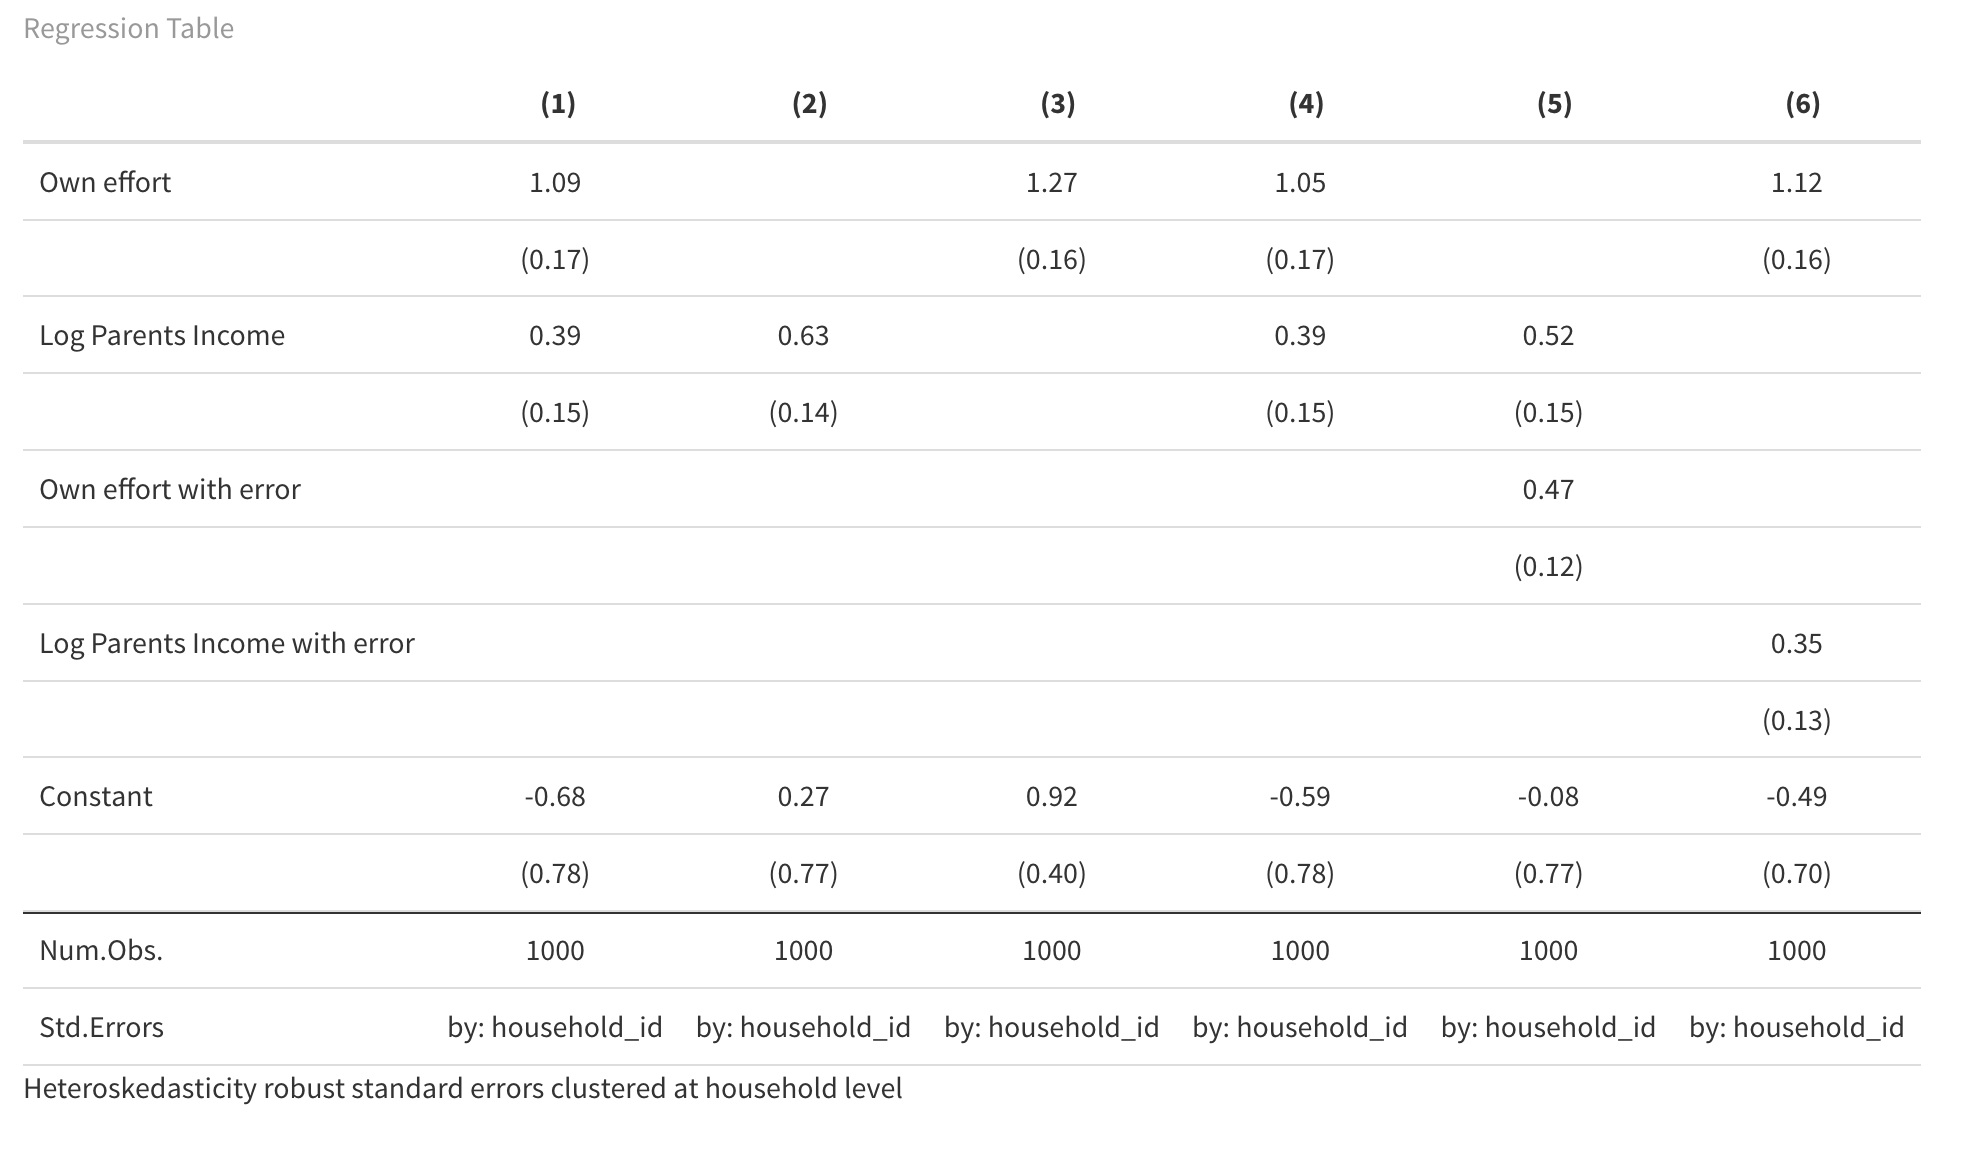
\includegraphics[width=18cm]{regression_table.png}

\subsection{モデル1の推定値の95\%信頼区間}

\begin{centering}
  \begin{gather}
    1.09 - 1.96 \times SE_{HAC}(\hat{\beta_1}) \le \hat{\beta_1} \le 1.09 + 1.96 \times SE_{HAC}(\hat{\beta_1}) \\
    1.09 - 1.96 \times 0.17 \le \hat{\beta_1} \le 1.09 + 1.96 \times 0.17 \\
    0.7568 \le \hat{\beta_1} \le 1.4232
  \end{gather}
\end{centering}

\begin{centering}
  \begin{gather}
    0.39 - 1.96 \times SE_{HAC}(\hat{\beta_2}) \le \hat{\beta_2} \le 0.39 + 1.96 \times SE_{HAC}(\hat{\beta_2}) \\
    0.39 - 1.96 \times 0.15 \le \hat{\beta_2} \le 1.09 + 1.96 \times 0.15 \\
    0.096 \le \hat{\beta_2} \le 0.684
  \end{gather}
\end{centering}

\end{document}



